\section{Wyświetlacz LCD}
\label{sec:lcd}
Do sygnalizacji wykonywanych czynności oraz polepszenia komunikacji pomiędzy
człowiekiem a robotem został wykorzystany wyświetlacz LCD. Użyty model to
wyświetlacz LCD 2x16, ze złączem pasującym do płyt systemu EVBXXX, z
podświetleniem biało-niebieskim. Element ten został wybrany ze względu na
stosunkowo niską cenę oraz możliwość podłączenia do płyty ewaluacyjnej EVBsam7s
wykorzystywanej podczas rozwoju robota.

Na wyświetlaczu pokazywane są czynności aktualnie wykonywane przez robota oraz
informacje pobierane z czujników zamontowanych na nim. Przykładowe komunikaty
pokazywane przez Dark Explorera mówią o: aktualnej temperaturze, ilości kroków
które wykonał użytkownik, kierunku w jakim podąża. Podłączony do robota
wyświetlacz pokazany jest na zdjęciu \ref{fig:LCD}.

\begin{figure}[!ht]
 \centering
 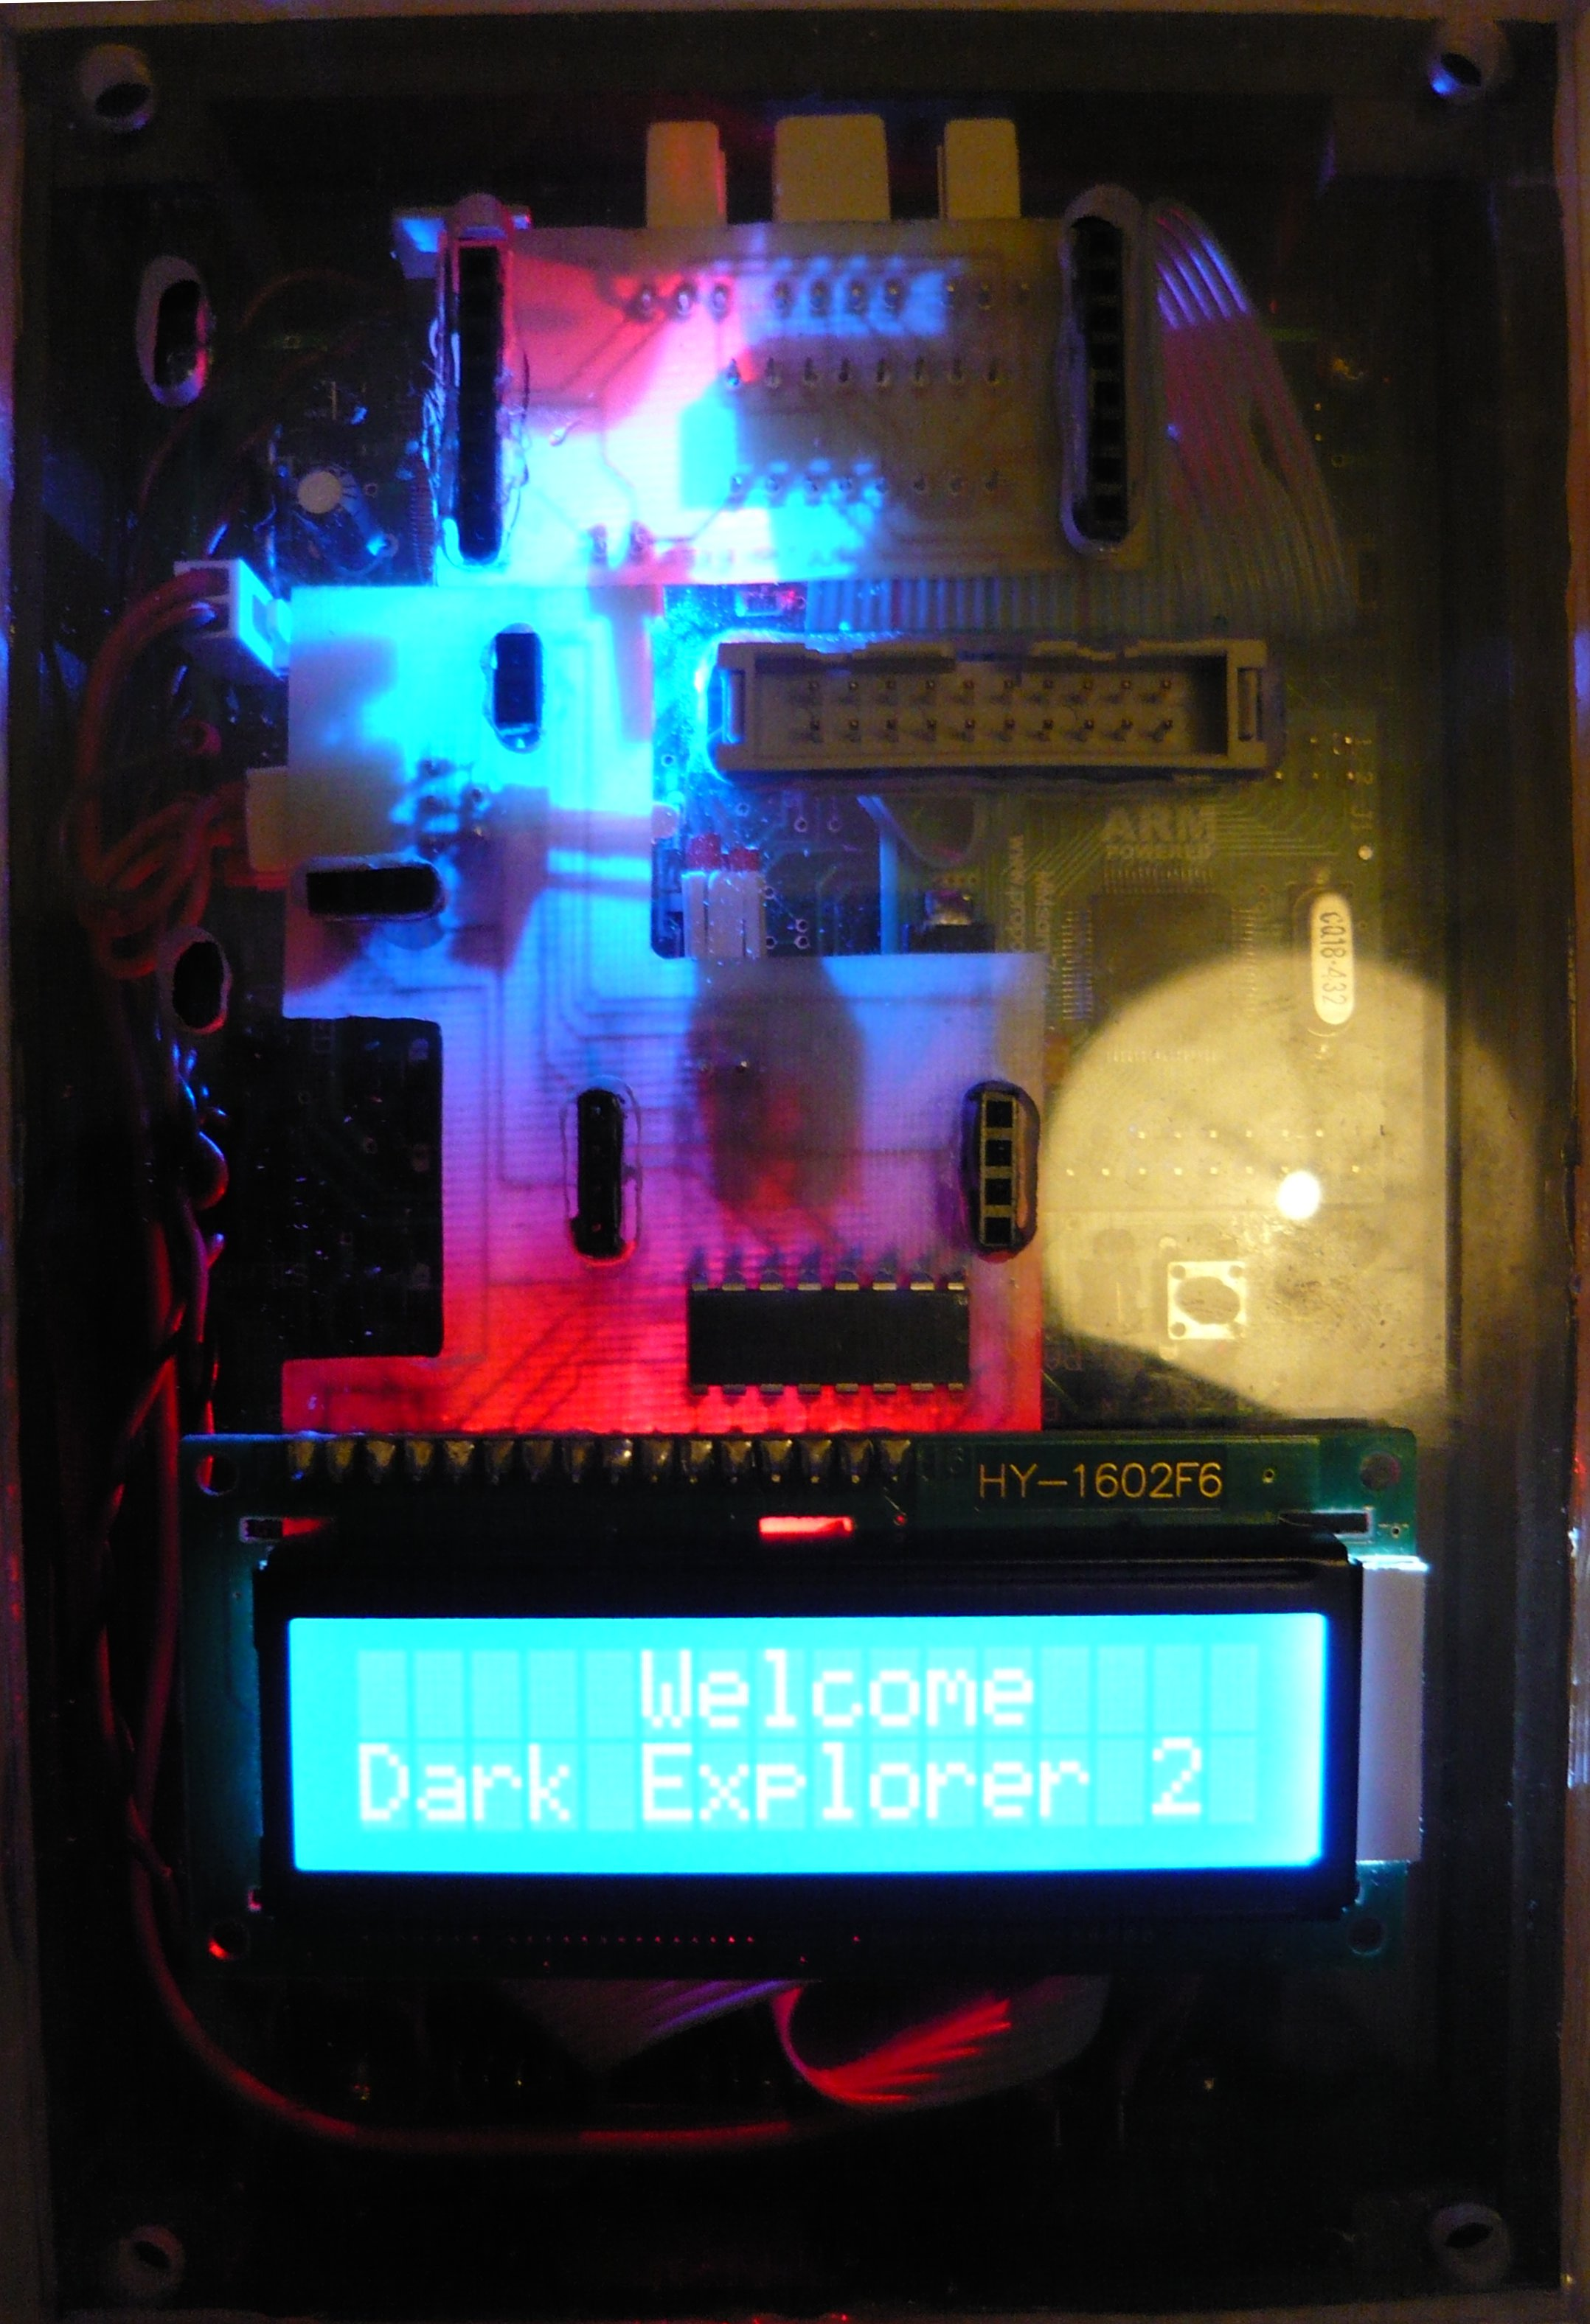
\includegraphics[height=100mm]{../images/ch04/lcd_welcome.jpg}
 \caption{Wyświetlacz LCD z komunikatem powitalnym}
 \label{fig:LCD}
\end{figure}

W celu wykorzystania wyświetlacza LCD konieczne było zastosowanie jakiegoś
sposobu na redukcję wejść oraz wyjść wykorzystywanych przez to urządzenie. W
konfiguracji podstawowej Dark Explorer udostępniał jedynie pięć złącz
GPIO\footnote{GPIO -- General Purpose Input/Output, złącza wejścia wyjścia
ogólnego przeznaczenia} natomiast sam wyświetlacz potrzebuje takich złącz sześć.

Z pomocą przyszedł tutaj 8-bitowy ekspander GPIO z interfejsem
$I^{2}C$\footnote{$I^{2}C$ -- szeregowa dwukierunkowa magistrala służąca do
przesyłania danych w urządzeniach elektronicznych}. Wykorzystany element to
PCF8574 firmy Philips. Układ ten posiada ośmio bitowy rejestr w~którym
przechowuje słowo odebrane poprzez interfejs $I^{2}C$. Każdy bit tego rejestru
jest odzwierciedlany jako stan wysoki lub niski na odpowiednich wyjściach GPIO. W
taki sposób możliwe jest sterowanie wyświetlaczem LCD. Wykorzystując ten pomysł
można znacząco rozszerzyć ilość portów GPIO na robocie i sterować dowolnymi
urządzeniami. Schemat płyty rozszerzeń z zaznaczonym modułem wyświetlacza LCD
widoczny jest na rysunku \ref{fig:ExBoardWithLCD}.

\begin{figure}[!ht]
 \centering
 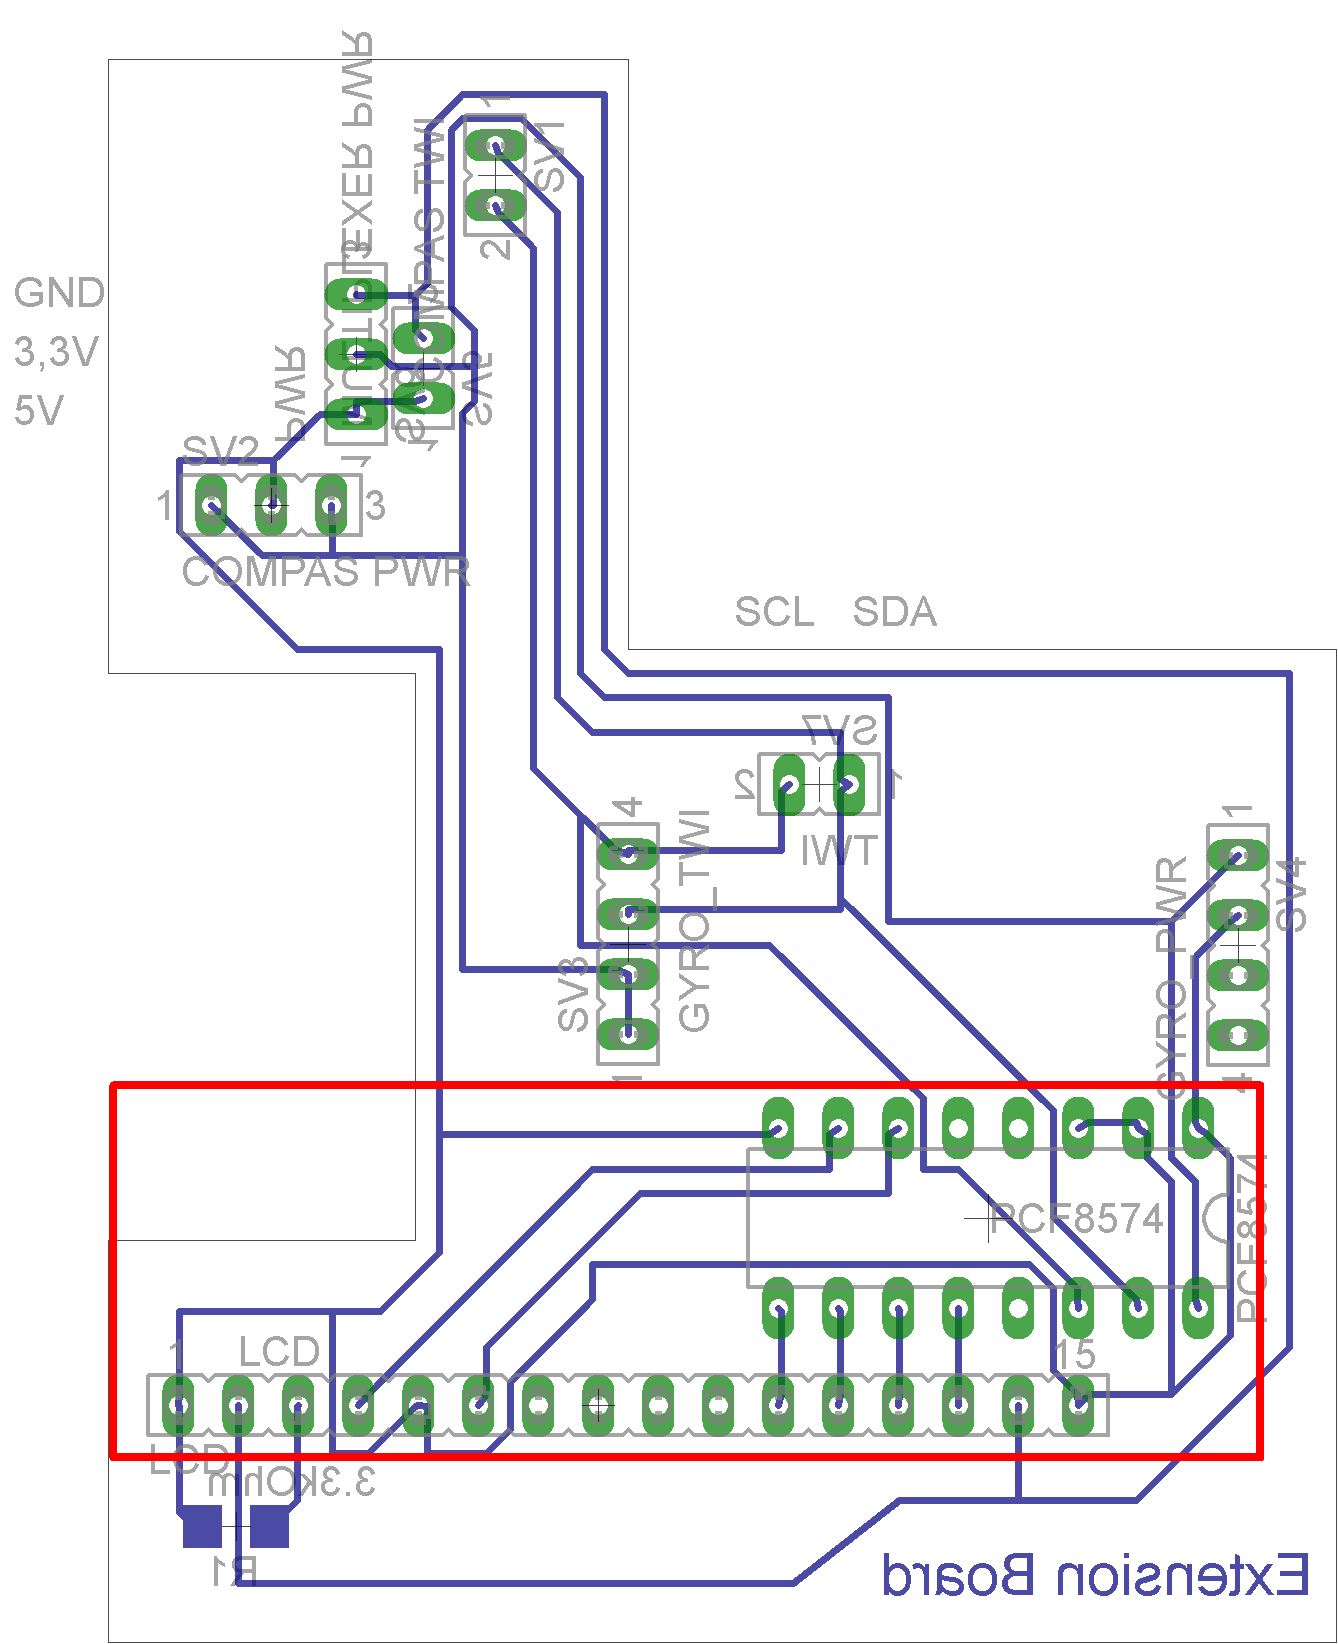
\includegraphics[height=125mm]{../images/ch04/extension_board-LCD.png}
 \caption{Layout cyfrowej części płyty rozszerzeń z zaznaczonymi elementami odpowiedzialnymi za obsługę wyświetlacza LCD}
 \label{fig:ExBoardWithLCD}
\end{figure}

Wyświetlacz został zakupiony jako moduł z wtykiem 16 pinowym. Można go podłączyć
do gniazda LCD na płycie rozszerzeń Dark Explorera.
